\begin{document}

\maketitle
\begin{frame}{Outline}
\setcounter{tocdepth}{1}
\tableofcontents
\end{frame}


\section{5 Themes}
\label{sec-1}
\begin{frame}[label=sec-1-1]{Humanity / Divinity of Christ}
\begin{itemize}
\item John 1  (NRSV) 1 In the beginning was the Word, and the Word was with God, and the Word was God. 2 He was in the beginning with God. 3 All things came into being through him, and without him not one thing came into being. What has come into being 4 in him was life, \ldots{}
\item Matthew 13:55 Is not this the carpenter’s son? Is not his mother called Mary? And are not his brothers James and Joseph and Simon and Judas?
\end{itemize}
\end{frame}

\begin{frame}[label=sec-1-2]{Spirit and Structure}
\begin{itemize}
\item Romans 8:2 For the law of the Spirit of life in Christ Jesus has set you free from the law of sin and of death.
\end{itemize}
\end{frame}

\begin{frame}[label=sec-1-3]{Reason and Revelation}
\begin{itemize}
\item Romans 16:25  Now to God who is able to strengthen you according to my gospel and the proclamation of Jesus Christ, according to the revelation of the mystery that was kept secret for long ages
\end{itemize}
\end{frame}

\begin{frame}[label=sec-1-4]{Works and Grace}
\begin{itemize}
\item 2 Timothy 1:9 who saved us and called us with a holy calling, not according to our works but according to his own purpose and grace. This grace was given to us in Christ Jesus before the ages began,
\end{itemize}
\end{frame}

\begin{frame}[label=sec-1-5]{Church and State}
\begin{itemize}
\item Romans 13 Let every person be subject to the governing authorities; for there is no authority except from God, and those authorities that exist have been instituted by God.
\end{itemize}
\end{frame}
\section{Philosophical issues}
\label{sec-2}
\begin{frame}[label=sec-2-1]{Battle of arguments for God}
\begin{block}{Anselm}
\end{block}
\begin{block}{Aquinas}
\end{block}
\begin{block}{Pascal}
\end{block}
\end{frame}
    {
    \usebackgroundtemplate{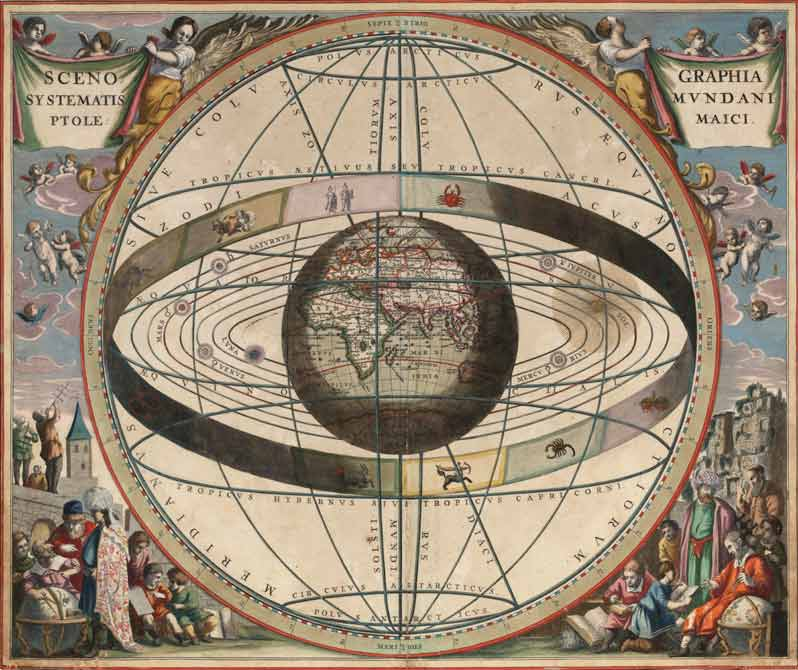
\includegraphics[height=\paperheight,width=\paperwidth]{./img/cellarius-ptolemaic-system.jpg}}
    \setbeamertemplate{navigation symbols}{}
    \begin{frame}[plain]
    \end{frame}
    }



    {
    \usebackgroundtemplate{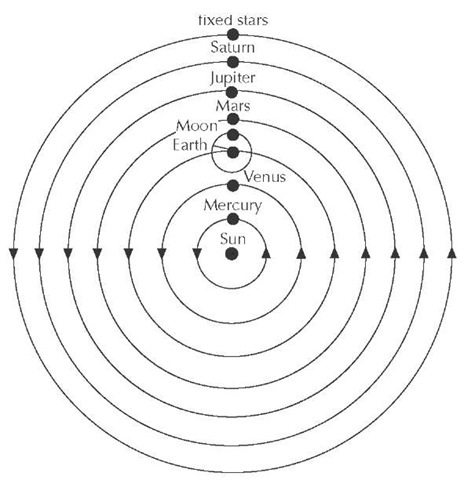
\includegraphics[height=\paperheight,width=\paperwidth]{./img/copernican.jpg}}
    \setbeamertemplate{navigation symbols}{}
    \begin{frame}[plain]
    \end{frame}
    }






\begin{frame}[label=sec-2-4]{Late Medieval Philosophy}
Ockham's razor argued the simpler explanation is to be preferred
\begin{block}{Realism}
\begin{itemize}
\item Universals are ``real''
\end{itemize}
\end{block}

\begin{block}{Nominalism}
\begin{itemize}
\item The only thing ``real'' are the names we put on things
\item Particulars are all that we experience and ``know''
\end{itemize}
\end{block}
\end{frame}

\begin{frame}[label=sec-2-5]{Nominalism \& Theology}
\begin{itemize}
\item Ockham (God can do anything)
\item 14th c. as focus of mysticism (Meister Eckhart)
\item Julian of Norwich (Mother Jesus)
\end{itemize}
\end{frame}

\begin{frame}[label=sec-2-6]{Protest against Church authority}
\begin{itemize}
\item Competing popes
\item Church offices for sale
\item John Wycliffe: the Bible could provide foundation to reform Church authority
\item John Hus: populist, all should receive communion, clergy are corrupt
\end{itemize}
\end{frame}
% Emacs 24.3.1 (Org mode 8.2.3c)
\end{document}
